\documentclass[11pt,a4paper]{report}
%\usepackage[left=2cm,top=2cm,right=2cm,bottom=2.5cm,nohead]{geometry}
%\setlength{\parindent}{0pt}
%\setlength{\parskip}{6pt}
\usepackage{graphicx}
\usepackage{rotating}
\usepackage{hyperref}
\usepackage{listings}
\usepackage{amsmath}
\usepackage{booktabs}
\usepackage{pdflscape}
\usepackage{afterpage}
\usepackage{capt-of}
\usepackage{rotating}
\usepackage{epstopdf}


\begin{document}

\begin{center}
{\huge ParFlow}\\
{\large Raphael Nussbaumer}\\
\today\\
\end{center}

\tableofcontents

\chapter{Introduction}
This manual was written during my Master where I learnt to use ParFlow (which, by the way, mean: ???). I will try to focus on very simple and obvious manipulation for new-user and some subtle tricks that I found quiet useful.

\section{What is ParFlow ?}
Developped at Lawrence Livermore National
Laboratory (LLNL), we can find on their \href{http://computation.llnl.gov/casc/parflow/parflow_home.html}{official ParFlow website}
\begin{quote}\it 
ParFlow is an integrated, parallel watershed model that makes use of high-performance computing to simulate surface and subsurface fluid flow. The goal of the ParFlow project is to enable detailed simulations for use in the assessment and management of groundwater and surface water, to investigate system physics and feedbacks and to understand interactions at a range of scales.
\end{quote}

\section{Some useful resources}
Before reading this manual, I strongly recommend to read the following resources (special the first one):
\begin{itemize}
\item The  \href{http://inside.mines.edu/~rmaxwell/parflow.manual.12-27-10.pdf}{Parflow user's manual (december, 2010)} will become your bedside book...
\item Professor Reed Maxwell website host the \href{http://inside.mines.edu/~rmaxwell/maxwell_software.shtml}{source file download link}(look also at his presentations on the website),
\item \href{http://parflow.blogspot.ca/}{Parflow blog} will help you to install ParFlow,
\item The original \href{http://computation.llnl.gov/casc/parflow/parflow_home.html}{parflow project website} gives some papers using PARFLOW
\item The \href{https://mailman.mines.edu/mailman/listinfo/parflow-users}{mailing list} can be used to ask questions 
\item And some other presentations :
\begin{itemize}
\item \href{http://www.umbc.edu/cuere/BaltimoreWTB/pdf/TR_2010_002.pdf}{The Baltimore exemple}
\item \href{https://www.google.ca/url?sa=t&rct=j&q=&esrc=s&source=web&cd=9&cad=rja&uact=8&ved=0CHUQFjAI&url=http%3A%2F%2Fcsdms.colorado.edu%2Fw%2Fimages%2FCyber_March_09_Maxwell.ppt&ei=owyIU63LJcjf8AGU34DQCQ&usg=AFQjCNH3lKFDUbs9GKHsIZyjGw3gIveTNg&sig2=qmeH_a8tHg33vPuFWiqNzw&bvm=bv.67720277,d.b2U} {ParFlow exemple}
\item \item {http://www.cosmo-model.org/content/tasks/workGroups/wg3b/meetings/2012-soilveg/COSMO-CLM2-ParFlow.pdf}{CLM presentations}
\end{itemize}
\end{itemize}

\chapter{Presentation of ParFlow}
In this introduction, we will try not to speak about computer. The first think you want to know is how does parflow think.\\
The idea of his designer is that Hydrological processes can't be represented as lumped "box" but that the spatial et temporal variation of each processes need to be represented as a continuum. (eg: Richards' equation is used in saturated AND unsaturated). To do this, a grid approach is necessary and only possible because of major advance in the computer science field. 

\section{Two solvers}
PARFLOW can run in two different mode:
\begin{itemize}
\item IMPES : steady state, fully saturated, single phase, 
\item RICHARDS : variably-saturated, transient conditions, overland flow and ability to be couple with CLM
\end{itemize}
As you can see, you certainly want to use Richards' solver for whatever you want to do...

\section{TCL/TK}

\href{https://en.wikipedia.org/wiki/Tcl}{TCL} stands for Tool Command Language, it is a \href{https://en.wikipedia.org/wiki/Scripting_language}{script language} which rather than compile, interpret and automate the execution of tasks that could alternatively be executed one-by-one by a human operator. (similar with a script in matlab ie:not a function)

Here is an exemple how to write TCL command in a file that has a '.tcl' extention
\begin{lstlisting}[language=TCL]
    # this is a comment
    set x 2
    set y 3
    set res [expr $x*$y]
    puts "2 * 3 is $res."
\end{lstlisting}

To run the file juste use the tclsh command in bash
\begin{lstlisting}[language=bash]
    $tclsh script.tcl 
\end{lstlisting}

You could also run line by line in the bash:
\begin{lstlisting}[language=bash]
    $ tclsh
    % commandName argument1 argument2
    % 
    % exit
\end{lstlisting}

Some rules:
\begin{itemize}
\item $[\quad]$: return the result of evaluating the script contained inside.
\item \$var return the value of the variable var
\item \href{http://www.tcl.tk/man/tcl/TclCmd/Tcl.htm}{more info on how to write TCL script}, \href{http://www.tcl.tk/man/tcl/TclCmd/contents.htm}{command list} and \href{http://www.tcl.tk/man/tcl8.5/tutorial/tcltutorial.html}{a tutorial}.
\end{itemize}

You can also run TCL from matlab but on my computer I add to recreate the \href{https://en.wikipedia.org/wiki/Environment_variable}{environment variable} \verb$PARFLOW_DIR$ and then run the script with the bang command (!)
\begin{lstlisting}[language=matlab]
    setenv('PARFLOW_DIR', '/home/raphael/parflow/parflow')
    !tclsh post.tcl
\end{lstlisting}

\section{Coupled}
One big strength of ParFlow is his ability to use CLM (\href{http://www.cesm.ucar.edu/models/cesm1.0/clm/CLM4_Tech_Note.pdf}{Common Land Model}) in a fully coupled fashion (like a module). This means that for each time step, it solves only one big matrix (not like two separate with an exchange flux). It avoid boundary condition errors and make the mode energy and mass conservative. CLM is part of the Land Surface Model (LSM) family (like \href{https://jules.jchmr.org/}{Jules}).
For info, Maxwell and Miller (2005) presents the first model (undistributed, not fully coupled) but the current version is the one describe in Kollet and Maxwell (2008).

It as also been coupled with the mesoscale atmospheric model ARPS. \href{http://igwmc.mines.edu/about/GWMI2010-01.pdf}{SLIM} is a Lagrangian, particle-tracking that can also be install with ParFlow.

\section{Multigrid}
Fully parallel, multigrid-preconditioned, finite difference/finite volume 3D flow
Multigrid method accelerate  the iterative solution by solving a coarse version of the version and using that to inform the fine grid solution (Ashby and Falgout, 1996) ( smooth to 1x1 → solve it, then 2x2x2 solve it … (interpolation)) . This is part of the preconditioner
Parralelism: (Falgout and Jones (1999))
the numerical algorithm (solver) must be scale linearly with problem size
Solver used is an Implicit method : Newton Methods 
Message passing – distributed memmory

\section{Which OS ?}
It can't be install on Windows but both Mac and Linux should work. You might want to consider to use a virtual box otherwise. But I would suggest to \href{http://www.everydaylinuxuser.com/2014/05/install-ubuntu-1404-alongside-windows.html}{install Ubuntu} (THE user-friendly Linux distribution) in a dual boot. Matlab, Visit, Python... what ever you would need are also available on Ubuntu.

Some
\begin{itemize}
\item ~ : home directory
\item ./ : current directory
\item ../: parent directory
\item the [tab] button auto-completes your typing on the command line.
\end{itemize}


\chapter{Installation}

\section{What is compilation}
What better than Wikipedia when you don't know something ?
\begin{quote} \it
A \href{https://en.wikipedia.org/wiki/Compiler}{compiler} is a program that transforms \href{https://en.wikipedia.org/wiki/Source_code}{source code} written in a programming language into another computer language. The most common reason for wanting to transform source code is to create an \href{https://en.wikipedia.org/wiki/Executable}{executable} program.
\end{quote}
It means than when you install a software, in order to run, the code of the software needs to be translate so that your \href{https://en.wikipedia.org/wiki/Operating_system}{OS} can understand it. On windows, the '.exe' does this job, but Linux has so many \href{https://en.wikipedia.org/wiki/Linux_distribution}{distributions} that we would need that many executable. 
On Ubuntu, \href{http://en.wikipedia.org/wiki/Advanced_Packaging_Tool}{apt-get} automaticaly retrieve, configure and install of software packages by compiling source code. The use of \href {http://en.wikipedia.org/wiki/Deb_(file_format)}{'.deb'} is the extension of the Debian software package format.

A lot of file appear that are the ingredient for the meal... what you need to find is the recipe : './configure'. This is an important script that check for the presence of the library required for the installation as well as creating the make file.
\begin{lstlisting}[language=bash]
    $./configure
\end{lstlisting}
If you just run ./configure, it will check that you have everything or will tell you what you need... Once it tells you that you're fine, just compile with make.
 \begin{lstlisting}[language=bash]
    $make
\end{lstlisting}
Once the compilation is finish run the executable with sudo make install
\begin{lstlisting}[language=bash]
    $sudo make install
\end{lstlisting}
As you will discover, compilation can be customize a lot with

http://stackoverflow.com/questions/10961439/why-always-configure-make-make-install-as-3-seperate-steps



\section{How to install it}
I used a lot what \href{http://parflow.blogspot.ca/)}{the blog} prescribe with some additional indication or explanation.

First, as suggested by John build a directory structure for your ParFlow installation called “parflow.” in home (or ~). Place all the things you download there. 

\subsection{Download and install compilers}
You need to install the tools to allows to compile with :
\begin{lstlisting}[language=bash]
    $sudo apt-get install build-essential
\end{lstlisting}

First, download and install the compilers (remember, the one that convert the source code to an executable for your machin) C, C++ and Fortran compilers and Tcl/Tk:
\begin{lstlisting}[language=bash]
    $sudo apt-get install gcc g++ gdc gfortran tcl-dev tk-dev
\end{lstlisting}



\subsection{Download Libraries}
\begin{itemize}
\item \textbf{Download OpenMPI}
\href{http://www.open-mpi.org/software/}{OpenMPI} is a \href{https://en.wikipedia.org/wiki/Message_Passing}{message-passing} system which rather than directly invoke a function by name (as in conventional programming), MP sends a \emph{message}. This powerfull tool allows separate program to work together. This is used when using parallel processor.

\item \textbf{Download SILO}: \href{https://wci.llnl.gov/codes/silo/downloads.html}{SILO} is a library for reading and writing a wide variety of scientific data to binary file. One of the more popular tools that process Silo data files is the \href{https://wci.llnl.gov/codes/visit/download.html}{VisIt visualization tool}.

\item \textbf{Download HYPRE}.\href{http://computation.llnl.gov/casc/hypre/software.html}{HYPRE} is a library for solving large, sparse linear systems of equations on massively parallel computers.
ParFlow

\item \textbf{Download ParFlow}, well you know who is \href{http://inside.mines.edu/~rmaxwell/maxwell_software.shtml}{PARFLOW}
\end{itemize}

\subsection{Install Libraries}
All the downloaded files are \href{http://en.wikipedia.org/wiki/File_archiver}{archive} which consits have been \href{http://en.wikipedia.org/wiki/Gzip}{compress ('.gz')} and  \href{(http://en.wikipedia.org/wiki/Tar_(file_format)}{combine ('.tar')}. To extract in command line use:
\begin{lstlisting}[language=bash]
    $tar -xvf FileName.tar.gz 
\end{lstlisting}

Here are two usefull idea of John:
You can also rename all the folder without the version number for simplicity.

And add \href{https://en.wikipedia.org/wiki/Environment_variable}{environmental variables} to Linux to have easier path. You can create a sort of global variable that will be accesible from everywhere in the shell. To do so add the following line in the \verb$~/.bash_aliases$ file.\href{https://en.wikipedia.org/wiki/Bash_(Unix_shell)}{Unix shell} executes this file when it start (\href{http://www.cyberciti.biz/tips/howto-linux-unix-bash-shell-setup-prompt.html}{here some tips})

\begin{lstlisting}[language=bash]
	$export CC=gcc
	$export CXX=g++
	$export FC=gfortran
	$export F77=gfortran

	$export PARFLOW_DIR=/home/john/parflow/parflow

	$export SILO_DIR=~/parflow/silo
	$export HYPRE_DIR=~/john/parflow/hypre
	$export PATH=$PATH:~/john/parflow/visit/bin
\end{lstlisting}

If you don't want to restart the shell, you can source the new file:
\begin{lstlisting}[language=bash]
    $source ~/.bash_aliases
\end{lstlisting}

Now, to install all the 4 libraries, you have to compile them as explain before. 
\subsubsection{Install OpenMPI}
\begin{lstlisting}[language=bash]
    $cd openmpi
    $sudo ./configure
    $sudo make all
    $sudo make check
    $sudo make all install
    $cd ..
 \end{lstlisting}
Compare to our theoretical example, we use \verb$make all$: this will compile not only the first \href{https://en.wikipedia.org/wiki/Make_(software)}{makefile} target but all of them. \verb$make check$ will runs post-build tests in the build directory.
 
\subsubsection{Install Silo} 
\begin{lstlisting}[language=bash]
    $cd silo
    $./configure --prefix=$SILO_DIR --disable-silex
    $make all
    $make check
    $make all install
    $cd ..
 \end{lstlisting}
 
 
\subsubsection{Install Hypre}
\begin{lstlisting}[language=bash]
    $cd hypre/src
    $./configure --prefix=$HYPRE_DIR --with-MPI [if you’re not using MPI, use --without-MPI]
    $make all
    $make check
    $make all install
    $cd ../..
 \end{lstlisting}

\subsubsection{Install ParFlow and PFTools, run the test cases}
Note: if you’re not using MPI, leave the last flag off.
\begin{lstlisting}[language=bash]
    $cd parflow/pfsimulator
    $./configure --prefix=$PARFLOW_DIR --enable-timing --with-clm --with-silo=$SILO_DIR --with-hypre=$HYPRE_DIR --with-amps=mpi1
    $make install
    $cd ../pftools
    $./configure --prefix=$PARFLOW_DIR --with-silo=$SILO_DIR --with-amps=mpi1
make install
    $cd ../test
    $sudo ldconfig
    $make check
 \end{lstlisting}

More importantly, before continuing we need to modify the Makefile to fix a few errors or else the installation will fail. Within the "config" folder, there exists a file called "Makefile.config"; locate it and open it in the editor of your choice. The changes we need to make happen in the LDLIBS specification near the bottom of the file. There are three changes to make: 
1) add a "-l" in front of "gfortran", 
2) remove the stray "-l", and 
3) remove the space between a "-l" and "gfortran".
This line cannot have any stray "-l" characters or anything that doesn't begin with "-l" or "-L", so if you're getting additional errors, check the LDLIBS line for any of those.
We've found that the configure script sometimes tries to link to a library as -lrt" (yes, it has a quotation mark hanging off the back) when using the Intel compilers and this will usually cause the installation to fail. If you see one or more flags in your LDLIBS line that includes a single quotation mark, just delete the entire flag.

\chapter{Conceptual Model}

This section is largely inspired by Kollet and Maxwell (2006)

\section{Water balance}
Largly exept for this section which come from Maxwell (2010)
\begin{equation}
\Delta S_{surface} + \Delta S_{subsurface} = Q_{precip} - Q_{runoff} + Q_{run-on} -ET -Q_{recharge} - Q_{S-out} + Q_{S-out}
\end{equation}

\begin{equation}
\Delta S_{surface} + \Delta S_{subsurface} = Q_{precip} - Q_{runoff} -ET
\end{equation}

\subsection{Richards' equation}

Need to have a look at : Jones and Woodward 2001 and 
Groundwater equation (steady-state, e.g. Ashby and Falgout 1996)


ParFlow use the 3D partial differential equation of Richards' equation. This equation enable to treat saturated and unsaturated within the same equations (i.e.: Variably saturated groundwater flow).
\begin{equation}
S_w(p)S_S\frac{\partial p}{\partial t} + \phi\frac{\partial S_w(p)}{\partial t} - \nabla \cdot \left\{ k_r\vec{k_s}\nabla \left(p -z\right)  \right\} = q_s
\end{equation}
where:
\begin{itemize}
\item $p$ is the pressure head $[L]$,
\item $z$ is the elevation $[L]$,
\item $S_w$ the water saturation , degree of saturation or relative saturation$[-]$ see Section~\ref{sec:degreeofsat}. It is usually represented by the Van Genuchten relationship (although ParFlow can use other relations)
\begin{equation}
S_w(p)=S_{res}+\frac{S_{sat}-S_{res}}{\left(1+(\alpha p)^n
\right)^{1-1/n}}
\end{equation}
	\begin{itemize}
		\item $S_{sat}$ relative saturated water content $[-]$,
		\item $S_{res}$ residual saturated water content $[-]$,
		\item $\alpha$ is a soil parameter $[L^{-1}]$
		\item $n$ is another soil parameter $[-]$
	\end{itemize}
\item $S_S$ specific storage coefficient $[L^{-1}]$,
\item $\phi$ the porosity$[-]$, 
\item $\vec{k_s}$ intrasect permeability tensor $[-]$,
\item $k_r$ is the relative permeability $[LT^{-1}]$,
\begin{equation}
k_r(p)=\frac{\left(1+\frac{(\alpha p)^{n-1}}{\left(1+(\alpha p)^n
\right)^{1-1/n}}\right)^2}{\left(1+(\alpha p)^n
\right)^{\frac{1-1/n}{2}}}
\end{equation}
\item $q_s$ is the water source/sink term $[T^{-1}]$
\end{itemize}
In ParFlow, and ParFlow uniquely, the physical quantity does not have a specific unit.So, be careful to remain consistent. For more information we coupled to CLM see section~\ref{sec:dealtime} .

Both \href{https://en.wikipedia.org/wiki/Dirichlet_boundary_condition}{Dirichlet} (first-type: pressure specified) and \href{https://en.wikipedia.org/wiki/Neumann_boundary_condition}{Neumann} (second-type: flow specified) boundary condition type can be used on all boundaries. Yet, for the ground boundary condition, Neumann is used with:
\begin{equation}
q_{BC} = \vec{K}(p)(\nabla p - z)
\end{equation}

\subsection{Overland Flow}
\label{subsec:overlandflow}


Overland is fully coupled with an flow boundary condition. This is explain in subsection~\ref{subsec:overlandflow}

Shallow overland flow is represented by the 2D-kinematic wave equation. Hydrostatic condition ($y=p$) is assumed and therfore the continuity equation is given by:
\begin{equation}
\frac{\partial p_s}{\partial t} = \nabla \cdot (\vec{v}p_s) +q_r+q_e
\end{equation} 
\begin{itemize}
	\item $p_s$ is the pressure head at surface $[L]$,
	\item $\vec{v}$ is the velocity at surface $[L T^{-1}]$. Using the kinematics wave approximation ($S_f=S_0$), Velocity can be calculated with Manning equation (cite)
	\begin{equation}
		v_{x,y}=\frac{\sqrt{S_{f,(x,y)}}}{n}p_s^{2/3}
	\end{equation}
	\begin{itemize}
		\item $n$ is the Mannings coefficient $[TL^{-2/3}]$
		\item $S_f$ is the friction slop $[-]$
	\end{itemize}
	\item $q_r$ is the source/sink term (rainfall, ET...) $[L T^{-1}]$
	\item $q_r$ is exchange rate with subsurface $[L T^{-1}]$
\end{itemize}


\subsection{Exchange flux}

Kollet (2006) introduced a general formulation to fully coupled the surface-subsurface system. This formulation eliminate numerical problem of the conductance type approach. 

A continuity in pressure ($p=p_s$) and flux ($q_{bc}=q_e$) between Richard's and the Kinematic wave is set up and the boundary condition is change. The overland equation can be re-written to gives the flux as:
\begin{equation}
q_e = \frac{\partial \| p,0\|}{\partial t} - \nabla \cdot (\vec{v}\| p,0\|)-q_r \\
\end{equation}
Which using the Neuman boundary condition gives:
\begin{equation}
-\boldsymbol{K}(p) \nabla (p - z) = \frac{\partial\| p_s,0\|}{\partial t} - \nabla \cdot (\vec{v}\|p_s,0\|) - q_r
\end{equation}

The $\| A,B\|$ operator choose the greater value between A and B. 

This formulation create the effect that the last cells is at the same time soil pressure and overland flow pressure

\begin{figure}[hbtp]
\caption{from Kollet (2006)}
\centering
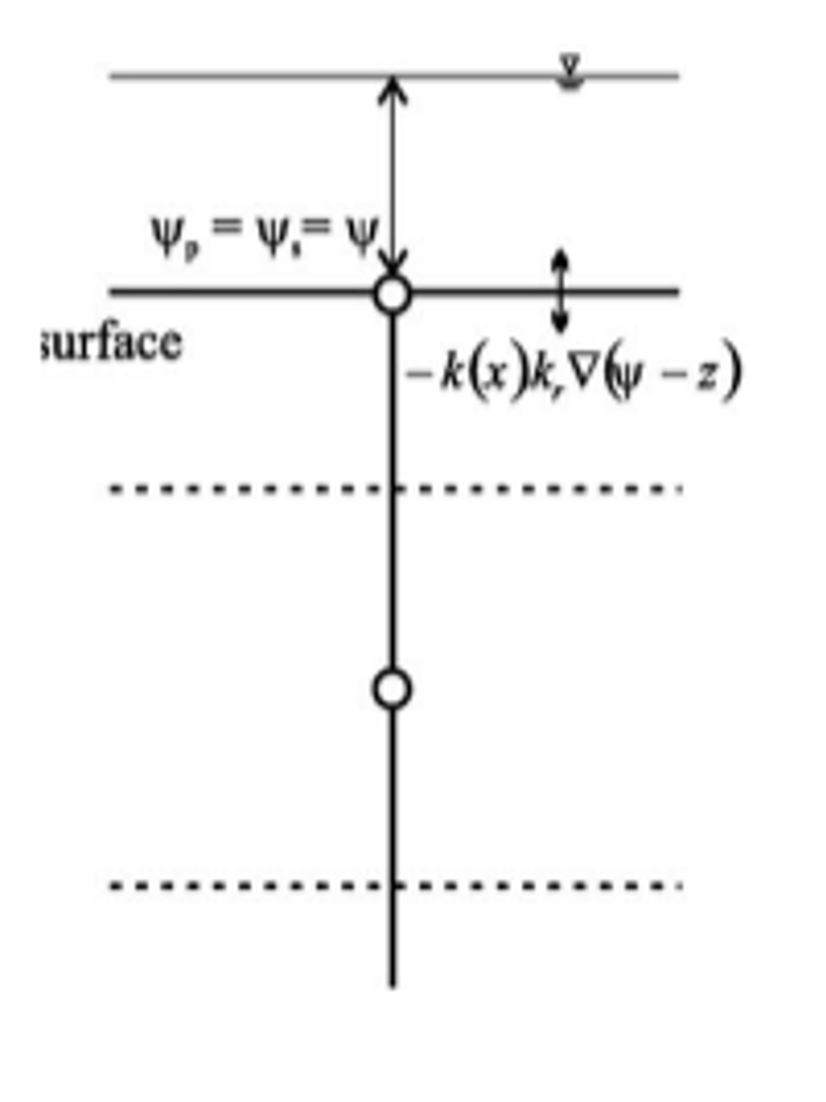
\includegraphics[width=0.5\textwidth]{bcflux.png}
\end{figure}






\section{Energy Balance}

This section is inspired by Kollet (2008) which explain how CLM is coupled to ParFlow.

\begin{equation}
R_n=H+L_vE_t+G
\end{equation}
\begin{itemize}
	\item $R_n$ is the net radiation $[W/m^2]$
	\begin{equation}
	R_n=S+L^{\downarrow}-L^{\uparrow}
	\end{equation}
	\begin{itemize}
		\item $S$ is the solar radiation $[W/m^2]$
		\item $L^{\downarrow}$ is the incoming Long-wave radiation $[W/m^2]$
		\item $L^{\uparrow}$ is the outgoing Long-wave radiation $[W/m^2]$
	\end{itemize}
	\item $H$ is the sensible heat $[W/m^2]$
	\begin{equation}
	H=H_c+H_g
	\end{equation}
	\begin{itemize}
		\item $H_c$ is sensible heat flux from vegetation $[W/m^2]$
		\item $H_g$ is sensible heat flux from ground $[W/m^2]$
	\end{itemize}
	\item $L_v$ is the latent heat of evaporation
	\item $E_t$ is total evaporation $[W/m^2]$
	\begin{equation}
	E_t=E_c+E_g=E_w+E_{tr}+E_g
	\end{equation}
	\begin{itemize}
		\item $E_c=E_w+E_{tr}$ is the evaporation from vegetation
		\item $E_g$ is the evaporation from the ground
		\item $E_w$  is the evaporation from wet foliage
		\item $E_{tr}$  is the transpiration
	\end{itemize}
	\item $G$ is the ground heat flux $[W/m^2]$, with $\lambda$ soi thermal conductivity and $T_{grnd}$ ground temperature
	\begin{equation}
	G=\lambda T_{grnd}
	\end{equation}
\end{itemize}

Mahfouf and Noilhan 1991 (alpha beta method)


\section{Surface Model: CLM}
Two fully coupled the water balence of equation ... and the energy balence of equation... the sink/source term relete with total evaportation $E_t$ and infiltration $q_g$:
\begin{equation}
q_s=L_vE_t + q_g
\end{equation}

All the energy term ($R_n, H, G$) are only depending on the water content ($\theta or S_w$) and with Van Genuchten at the pressure $p$ which is share by PF to CLM.

Yet, few assumptions/simplifications are done:
\begin{itemize}
\item Independance of hydraulic conductivity $k_r$ and temperature $T$.
\item neglect the convective component in the ground heat flux
\item neglecting explicit vapor transport in ground evaporation.
\end{itemize}










\chapter{Numerical Implementation}
I will try to explain or at least gather the information to describe the numerical method used.

Parflow is using \textit{"...an implicit backward Euler and cell-centered finite difference scheme for the discretization in time and space respectively. The equations are solve using a Newton-Krylov method with multigrid preconditioning"(Kollet, 2008)}.

\section{Numerical method to solve PDE}
The general expression of an partially differential equations (PDE) is given as follow where the highest derivated degree is the order of the PDE (first:$\frac{\partial u}{\partial x_1}$ and second:$\frac{\partial^2 u}{\partial x_1 \partial x_n}$)
\begin{equation}
F \left (x_1, \ldots, x_n, u, \frac{\partial u}{\partial x_1}, \ldots, \frac{\partial u}{\partial x_n}, \frac{\partial^2 u}{\partial x_1 \partial x_1}, \ldots, \frac{\partial^2 u}{\partial x_1 \partial x_n}, \ldots \right) = 0
\end{equation}

The Finite methods are numerical technique for finding approximate solutions of PDEs.

\subsection{Finite Difference Method (FDM)} \href{https://en.wikipedia.org/wiki/Finite_difference}{Finite Difference method} (FDM) uses \href{http://en.wikipedia.org/wiki/Finite_difference}{finite difference} equations to approximate derivatives. see section~\ref{Numerical_method_to_solve_ODE}
\subsection{Finite Volume Method (FVM)} \href{https://en.wikipedia.org/wiki/Finite_volume_method}{Finite Volume method} (FVM) uses the \href{https://en.wikipedia.org/wiki/Divergence_theorem}{Divergence theorem} at each node considered as a volume. FDM is a special case of FVM.
\subsection{Finite Element Method (FEM)}
\href{https://en.wikipedia.org/wiki/Finite_element_method}{Finite Element method} (FEM) is transforming the PDE into a system of simple function. It uses variational methods (the calculus of variations) to minimize an error function and produce a stable solution.


\subsection{Numerical method to solve ODE}
\label{Numerical_method_to_solve_ODE}
The general expression of an ordinary differential equations (ODE) is given as follow where $n$ is the order
\begin{equation}
F(x,y,y',y'',...y^{(n)})=0
\end{equation}

\begin{itemize}
\item an the \href{https://en.wikipedia.org/wiki/Euler_method}{Euler Method} is a numerical procedure to solve ODE of the first order ($n=1$) given an initial condition with:
\begin{equation}
y_{n+1}=y_n+(x_{n+1}-x_n)f(x_n,y_n)
\end{equation}
\item \href{https://en.wikipedia.org/wiki/Explicit_and_implicit_methods}{Implicit vs explicit}: Explicit methods calculate the state of a system at the next time from the state of the system at the current time (ie: $y_{n+1} = f(y_n)$), while implicit methods find a solution by solving an equation involving both the current state of the system and the later one (ie: $g(y_{n+1},y_n)=0$).

\item \href{}{Backward vs forward}: are form of the finite difference expression. They differ in the choice of the node choose to solve the derivate.
\begin{subequations}
forward, central and backward:
\begin{align}
        \left. \frac{d y}{d x}\right|_n=\frac{y_{n+1}-y_n}{\Delta x} \\
        \left. \frac{d y}{d x}\right|_n=\frac{y_{n+1}-2y_n+y_{n-1}}{2\Delta x} \\
		\left. \frac{d y}{d x}\right|_n=\frac{y_{n}-y_{n-1}}{\Delta x}
\end{align}
\end{subequations}
As you must have notice, backward is a type of explicit and forward a type of implicit method. (they are not the same thing !)
\item The \href{https://en.wikipedia.org/wiki/Backward_Euler_method}{implicit backward Euler method} computes the approximation:
\begin{equation}
y_{n+1} = y_n +(x_{n+1}-t_n) f(x_{n+1},y_{n+1})
\end{equation}
As you can see in this equation the term $y_{n+1}$ appear in both side which make it implicit.

\item Space and time: In the case where there is two \href{https://en.wikipedia.org/wiki/Dependent_and_independent_variables}{independent variables} ($x_1,x_2$ or $x,t$), the equation to solve is a \href{https://en.wikipedia.org/wiki/Partial_differential_equation}{partial differential equation} (PDE) ($F(x,t,y,\frac{dy}{dx},\frac{dy}{dt})=0$) . The approximation can therefore be different for space and time. In our case we have:
\begin{subequations}
\begin{align}
        \left. \frac{d y}{d t}\right|_n=\frac{y_n-y_{n-1}}{\Delta t} \\
        \left. \frac{d y}{d x}\right|_n=\frac{y_{n+1}-2y_n+y_{n-1}}{2\Delta x} \\
\end{align}
\end{subequations}
\end{itemize}



\section{Newton and Kyrlov method}
The Newton method is used to solve the equation (Euler method give an approximate equation to solve, Newton solves it !). In the general term, solving mean find $u$ such as $F(u)=0$. (the $u$ term would be in our case $y_{n+1}$) A description of the Newton method:
\textit{"one starts with an initial guess, then the function is approximated by its tangent line (derivate), and one computes the x-intercept of this tangent line. This x-intercept will typically be a better approximation to the function, and the method can be iterated."}
In another word : 
\begin{equation}
x_{k+1}=x_k-\frac{f(x_k)}{f'(x_k)}
\end{equation}


If we want to go one step futher, we need some other tools such as the \href{https://en.wikipedia.org/wiki/Jacobian_matrix_and_determinant}{Jacobian matrix} which gather all the different derivate of an \href{https://en.wikipedia.org/wiki/Vector-valued_function}{vector function} $F=[F_1(x_1,...,x_n),...,F_m(x_1,...,x_n)]$  in the following way:
\begin{equation}
J=\begin{bmatrix} \dfrac{\partial F_1}{\partial x_1} & \cdots & \dfrac{\partial F_1}{\partial x_n} \\ \vdots & \ddots & \vdots \\ \dfrac{\partial F_m}{\partial x_1} & \cdots & \dfrac{\partial F_m}{\partial x_n}  \end{bmatrix}.
\end{equation}

Using this the Newton method can be upgrade for vector function which appear to be a linear system ($Ax=b$ where $A=J(x)$, $dx=x$ and $-F(x)=b$)
\begin{equation}
J(x)dx=-F(x)
\end{equation}

In order to find the Jacobian matrix, numerical approximation are often required (such as finite difference seen before). Yet this computations involve a lot of computation and memory and therefore approximation of the Jacobian is often used.

Krylov method is solving a linear system ($Ax=b$) in an iterative way which requires only matrix–vector products (not individual element) to carry out the iteration. In 2004, Knoll and Keyes(ref: ) reviewed the Jacobian-free Newton-Krylov method (JFNK) which is used in Parflow. I can't go in more detail because I don't fully understand. Google it if you want to know more.


\section{Preconditioning}
Th last notion  that we are going to talk about is the preconditioning. It is a procedure to condition a given problem into a form that is more tractable 


\href{https://en.wikipedia.org/wiki/Multigrid_method}{Multigrid} methods accelerate the iterative solution by solving a coarse version of the problen and using using that to inform the fine grid.

could be a
Harmonic weighting and a one point-upstrean weighting of the relative permeabilites (Kellet,2006, p949).
 finite difference/finite volume 3D flow


Jones and Woodward (2001)


\section{Parralelism}
: (Falgout and Jones (1999)) ashby and Falgout 1996
the numerical algorithm (solver) must be scale linearly with problem size
Message passing – distributed memmory
using a \href{http://en.wikipedia.org/wiki/Octree}{Octree}  data structure


Conclustion:
speed up : generally 10x faster than 2D and 100x for 3D























\chapter{Revised Guide of a PARFLOW script}

In this chapter, I will go through all the step to create the different input file. 

\section{Scheme of the grid}
The Figure~\ref{fig:grid} displays a sample grid illustrating all the grid information. I would like to draw you attention to the following points:
\begin{itemize}
\item It is a cell-center scheme. ($x_1=dx/2$)
\item The land surface stop at the center of the cell while the water table (when p>0)is between two cell. 
\item the overland flow occur in half of the last cell. But all the cell above are inactive(eventhough their is pond-water in them)
\item CLM run over the ten first cell whatever grid resolution there is.
\end{itemize}
\begin{figure}[hbtp]
\caption{2D exemple of a grid}
\label{fig:grid}
\centering
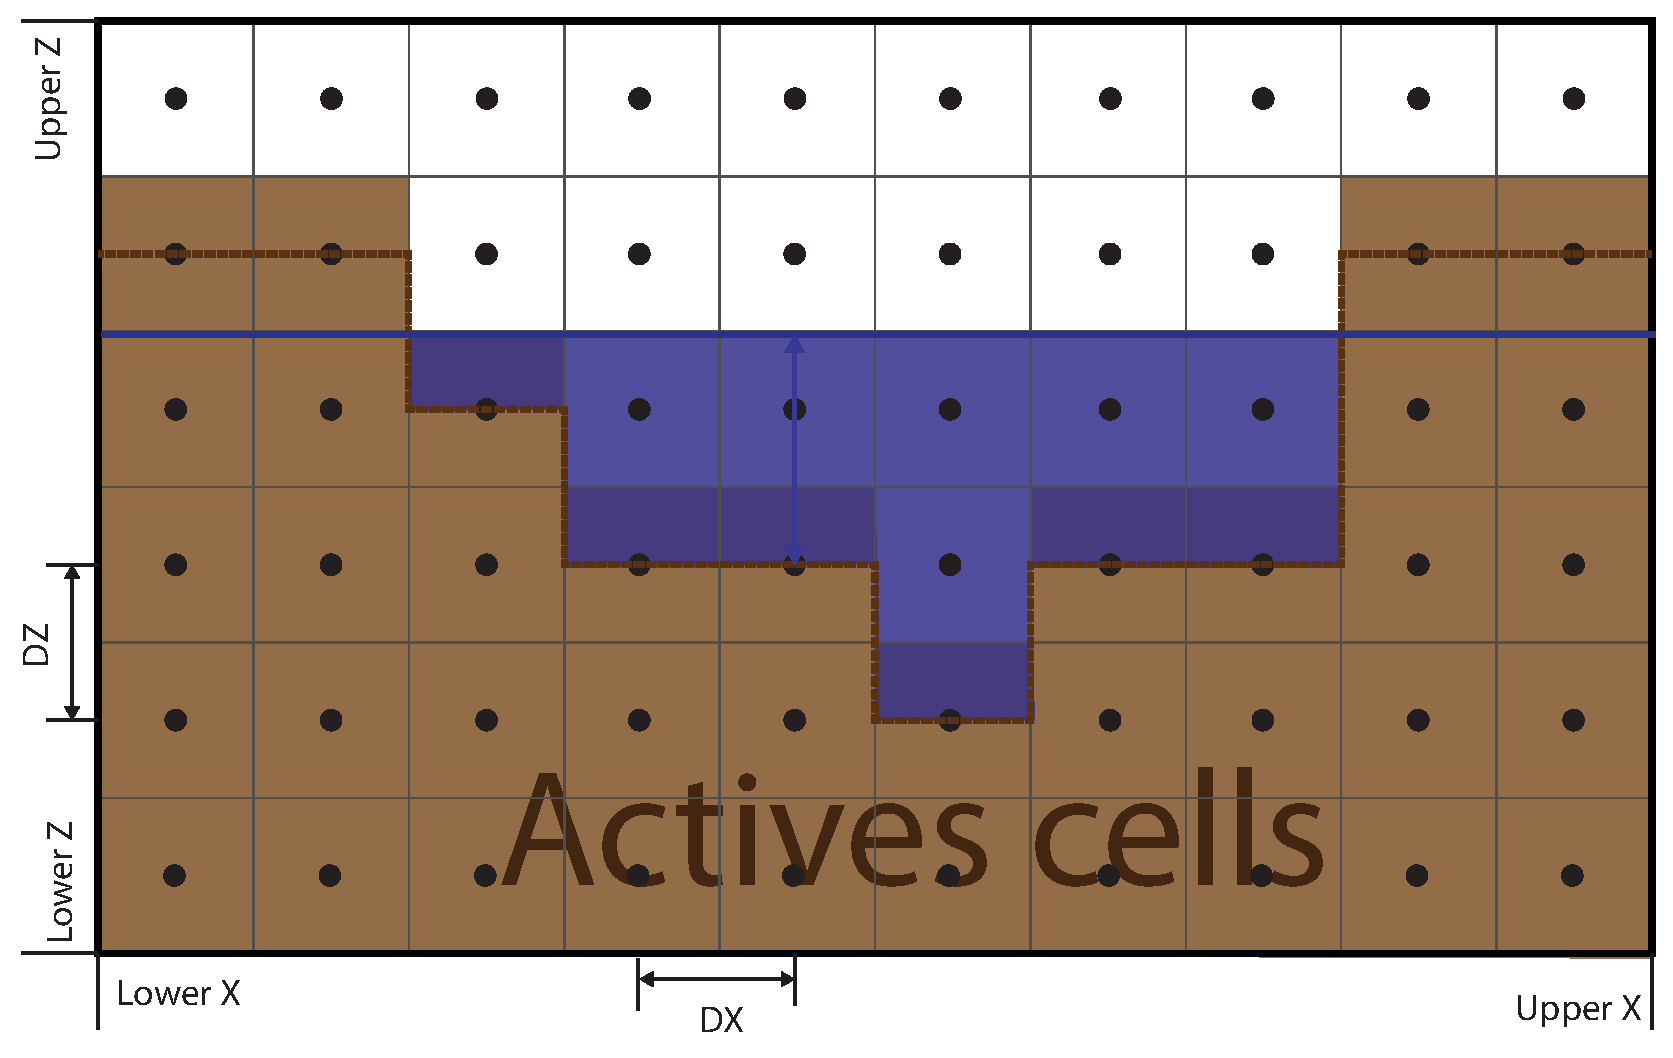
\includegraphics[width=\textwidth]{GRID.eps}
\end{figure}


\section{Summury of Input/Ouput}

Table of input output

\begin{landscape}
\begin{table}[htbp]
\centering
\begin{tabular}{llp{10cm}ll}
\toprule
 Key     & Symbole      & Description                                                       & Unit & type             \\
\midrule
\multicolumn{5}{c}{\emph{Grid Information}}                                                                \\
Lower X,Y,Z & &position of the origin                                            &  & double           \\
NX,NY,NZ   & & number of grid cells                                              & & integer          \\
DX,DY,DZ  &  & size of a grid cells& [$L$]                                       & double           \\
\multicolumn{5}{c}{\emph{Surface Information}}                                                             \\
shape     & & mesh of the surface shape built with \verb$ ...$)                                          & .pfsol             \\
slope x, y & & value of the slope can be build with \verb$pfslopex$ by PF from DEM (3D not 2D) & & 2D-pfb or double \\
manning  &$n$ & value of the manning coefficient &[$-$]                           & 2D-pfb or double \\
\multicolumn{5}{c}{\emph{Soil information}                                                               } \\
perm     & $ k_r $  & saturated hydraulic conductivity& [$L/T$]                         & 3D-pfb or double \\
porosity   &$\phi$ & porosity of the soil                                              &[-] & double           \\
alpha, n   & $\alpha$, $n$ & parameters for Van Genuchten if 3D, needs to be on domain& [$?$]                      & double or 3D-pfb         \\
SRes, SSat  & $S_{res}$, $S_{sat}$ &                                                                  Saturated water content (see subsection~\ref{sec:degreeofsat}) & [-] & double or 3D-pfb          \\
\multicolumn{4}{c}{\emph{Met forcing}}                                                                     \\
DSWR   & $L^{\downarrow}$ & Long wave radiation incoming&[$W/m^2$] & 1D-t             \\
DLWR   & $K^{\downarrow}$ &Short wave radiation incoming&[$W/m^2$] & 1D-t             \\
APCP     & $P$   & Precipitation &[$mm/s$]                                           & 1D-t             \\
Temp     & $T_a$   & Air temperature & [$K$]                                            & 1D-t             \\
UGRD   && N-S wind speed & [$m/s$]                                      & 1D-t             \\
VGRD   && E-W wind speed & [$m/s$]                                      & 1D-t             \\
Press     &  & Atmospheric Pressure & [$Pa$]                                      & 1D-t             \\
SPFH      &  & Specific humidity & [$kg/kg$]                                      & 1D-t    \\
\bottomrule        
\end{tabular}
\end{table}


\begin{table}[htbp]
\centering
\begin{tabular}{llcp{7cm}cl}
\toprule
 function & Key           & Symbole & Description                                                       & Unit & type             \\
 \midrule
\multicolumn{6}{c}{\emph{Grid Information}}                                                                \\
\verb$WriteSiloMask$ & mask && matrix of 1 (soil) and 0 (air)                                            &  & 3D-0T         \\
\verb$pfcomputetop mask$ & top    && matrix of the top soil elevation                                              & & 2D-0T         \\
\verb$pfextracttop 3Dfield$ & top-layer    && extract the ground value for any 3D field (can be loop over time) & & 2D-0T         \\
\multicolumn{6}{c}{\emph{CLM output}}    \\
\verb$WriteSiloCLM$&\verb$eflx_lh_tot$     & $Lv$ & latent heat flux total & $[W/m^2]$ &    3D-0NT \\
\verb$WriteSiloCLM$&\verb$eflx_lwrad_out$   & $L^{\uparrow}$  & outgoing long-wave radiation & $[W/m^2]$ &    3D-NT \\
\verb$WriteSiloCLM$&\verb$eflx_sh_tot$   & $H $  & sensible heat flux total & $[W/m^2]$ &    3D-0NT \\
\verb$WriteSiloCLM$&\verb$eflx_soil_grnd$   & $ H_g$   & ground heat flux & $[W/m^2]$ &    3D-0NT \\
\verb$WriteSiloCLM$&\verb$qflx_evap_tot$   & $L_vE_t$   & total evaporation & $[W/m^2]$ &    3D-0NT \\
\verb$WriteSiloCLM$&\verb$qflx_evap_grnd$   &  $L_vE_g$  & ground evaporation without sublimation & $[mm/s]$ &    3D-0NT \\
\verb$WriteSiloCLM$&\verb$qflx_evap_soi$   &   & soil evaporation & $[mm/s]$ &    3D-0NT \\
\verb$WriteSiloCLM$&\verb$qflx_evap_veg$    & $L_vE_c$  & vegetation evaporation & $[mm/s]$ &    3D-0NT \\
\verb$WriteSiloCLM$&\verb$qflx_tran_veg$  & $ E_{tr}L_v$  & vegetation transpiration & $[mm/s]$ &    3D-0NT \\
\verb$WriteSiloCLM$&\verb$qflx_infl$   & $q_g$   & soil infiltration & $[mm/s]$ &    3D-0NT \\
\verb$WriteSiloCLM$&\verb$swe_out$  & $S $   & snow water equivalent & $[mm]$ &    3D-0NT \\
\verb$WriteSiloCLM$&\verb$t_grnd$  & $T_g$   & ground surface temperature & $[K]$ &    3D-0NT \\
\verb$WriteSiloCLM$&\verb$t_soil$   & $T_s$  & lsoil temperature over all layers & $[K]$ &    3D-0NT \\
\multicolumn{6}{c}{\emph{PF ouput}}    \\
\verb$WriteSiloSubsurfData$&pressure   & $Press $  & pressure & $[L]$ &    3D-NT \\
\verb$WriteSiloSubsurfData$&saturation  & $S $  & saturation ($S_{res}<S<S_{sat}$) & $[-]$ &    3D-NT \\
\verb$pfhhead pressure$ &head &   $H$  & head (P+z) & $[L]$ &    3D-NT \\
\verb$pfflux perm head$ &flux &   $q$  & Darcy flow & $[L/T]$ &    3D-NT \\
\multicolumn{6}{c}{\emph{PF computed}}    \\
\verb$pfsubsurfacestorage ...$ &surface runoff   & $R $  & runoff out of domain & $[L^3/T]$ &    3D-NT \\
\verb$pfsurfacestorage ...$ &surface storage   & $SS $  & surface water storage (ponding) & $[L^3]$ &    3D-NT \\
\verb$pfsurfacerunoff ...$ &subsurface storage &   $SSS$  & sub-surface water storage & $[L^3]$ &    3D-NT \\
\verb$pfsum ...$ & &     & sum of any 2D or 3D field & $[L^3]$ &    0D\\
\bottomrule
\end{tabular}
\end{table}

\end{landscape}









 \section{Architecture of files}
In an very unstructure manner, PARFLOW find the input and output on folder (where the main script is ). But like me I encourage you to structure a little bit more your data.
\begin{itemize}
\item \verb$Pre/$ is the folder containing the preparation step for the data
	\item \verb$Required_data/$: is the folder with external data (DEM, met forcing)
	\item \verb$pre.m$: is the matlab script to create the input data.
	\item \verb$generate_function/$: folder with all the matlab function which generate data
	\begin{itemize}
		\item \verb$generate_dem()$:
		\item \verb$generate_soil()$:
		\item \verb$generate_met()$:
		\item \verb$generate_dem()$:
	\end{itemize}
	\item \verb$Input/$: is the folder with all the file required for the TCL script produced by my preparations steps. Parflow will then just copy these file into in main folder
	\item \verb$Output/$: is the folder where the run will create all the new data
	\begin{itemize}
		\item \verb$TXT$:
		\item \verb$CLM output$:
	\end{itemize}
	\item \verb$Post/$: 
	\begin{itemize}
		\item \verb$load_data()$:
		\item \verb$open_SA()$:
		\item \verb$plot$:
	\end{itemize}
	
\end{itemize}


\section{Various notes and remarques}


\begin{itemize}
\item I was not able to make this expression work for decimal value (even with transforming into double)
\begin{lstlisting}[language=TCL]
set DY	[expr ($UpperY - $LowerY) / $NY]
\end{lstlisting}

\item For all the .SA file imported it is mandatory to set the grid for them like this
\begin{lstlisting}[language=TCL]
pfsetgrid {nx ny nz} {x0 y0 z0} {dx dy nz} {x0 y0 z0} {dx dy dz} $dem
\end{lstlisting}

\item There is a nice little option with the solver: 
\begin{lstlisting}[language=TCL]
Pfset Solver.TerrainFollowingGrid		True
\end{lstlisting}






\item 	
\end{itemize}

\section{CLM files}
Fours files are necessary for CLM:
\begin{itemize}
	\item \verb$drv_vegp.dat$: vegetation parameter data file 
	\item \verb$drv clmin startup dat$: CLM parameters see CLM manual :Appendix 4: IGBP Land Cover Types Definition. ParFlow only allows one land cover type per grid cell: there should be one column per row with a value of 1.0, and all other values of 0.0. Sand and clay were previously used for the hydrology part of CLM, but have been replaced by ParFlow, and so dummy values are used. 
	\item \verb$drv_vegm.dat$: specify vegetation type 
	\item \verb$narr_1hr.tx$ tMeteorological Forcings ()
\end{itemize}

	
	
\begin{itemize}
\item Sand and clay were previously used for the hydrology part of CLM, but have been replaced by ParFlow, and so dummy values are used. (about \verb$drv_vegm.dat$)

\item There should be one column per row with a value of 1.0, and all other values of 0.0. This is because ParFlow only allows one land cover type per grid cell.

\item The ending time can be set far in the future, because the simulation ending time is controlled by ParFlow (\verb$drv_clmin.dat$)

\item For the CLM files, manual distribution of the file need to be done
\begin{lstlisting}[language=TCL]
set num_processors [expr [pfget Process.Topology.P] * [pfget Process.Topology.Q] * [pfget Process.Topology.R]] 
for {set i 0} { $i <= $num_processors } {incr i} { 
	file delete drv_clmin.dat.$i 
	file copy drv_clmin.dat drv_clmin.dat.$i 
}
\end{lstlisting}
\end{itemize}









\section{Deal with Sres and Ssres}
\label{sec:degreeofsat}

\begin{table}[htbp]
\centering
\begin{tabular}{p{4.5cm}cll}
\toprule
Name 		& Symbol 		& Definition 			& Equation \\
\midrule
Porosity		& $\phi [\%]$	& void over total		& $ \eta=\frac{V_v}{V_t} $ \\
Water content		& $\theta [\%]$	& water over total		& $\theta=\frac{V_w}{V_t}$ \\
Water saturation		& $S_w [\%]$	& water over void		& $S_w=\frac{V_w}{V_v}=\frac{\theta}{\eta}$ \\
Normalized water content	 or effective saturation 	& $\Theta$ or $S_e [\%]$	&  & $\Theta=\frac{\theta -\theta_{res}}{\theta_{sat} -\theta_{res}}$ \\
\bottomrule
\end{tabular}
\end{table}

In theory, $\theta_{res}$ is the residual water content, defined as the water content for which the gradient $d\theta/dh$ becomes zero; and, $\theta_{sat}$ is the saturated water content, which is equivalent to porosity, $\phi$. In practice, we fit the Van Genuchten curve to data and find these parameters.

As a note, the \verb$pfwatertabledepth$ function of ParFlow computes, as explain in the manual the distance from the top to first cell with saturation=1. First, this isn't right in my opinion as the water-table should be computed from the first cell where pressure=0, and secondly, when you put a saturated water content less than 1, this function is not working. (So don't use it)










\section{Deal with Specific humidity}
The mass of air ($m_a$) is the sum of a mass of vapor ($m_v$) and all the other molecules (mainly N$_2$ and O$_2$) that form the dry mass ($m_d$).
\begin{equation}
m_a=m_v+m_d
\end{equation}

\begin{itemize}
 \item The \emph{mixing ratio} is the ratio of vapor mass over dry mass.
   \begin{equation}
 \mathrm{MR} = \frac{m_v}{m_d}
 \end{equation}


 \item The definition of \emph{Specific humidity} is the ratio of mass of vapor over mass of air (value around 0.01). 
  \begin{equation}
 \mathrm{SH} = \frac{m_v}{m_a}
 \end{equation}
 
 \item More often the \emph{relative humidity} is often used. In this case humidity is the ratio of mixing ratio of the air over the mixing ratio of the same air brought to saturation of water. With is the same as the ratio of specific humidity over saturated specific humidity
 \begin{equation}
 \mathrm{RH} = \frac{P_v}{P_v^{sat}} = \frac{\mathrm{MR}}{\mathrm{MR}^{sat}}
 \end{equation}
 
\end{itemize} 
 
 How to convert between them ? 
First, as the mass of vapor is so small compare to the mass of air, it is commonly assumed that:
\begin{equation}
\mathrm{SH} = \frac{m_v}{m_d +m_w} = \frac{\mathrm{MR}}{1+\mathrm{MR}} \approx \mathrm{MR}
\end{equation}

 From Dalton's law, (total) pressure is equal to the sum of partial pressure ($P_a=P_v+P_d$) where each partial pressure is proportional to the his molar ratio (with $M_d = 0.028964$ and $M_w=0.018016$ are the molecular weight [$kg/mol$]):
 \begin{equation}
 \frac{P_v}{P_a}=\frac{n_v}{n_a}=\frac{m_v/M_v}{m_v/M_v + m_d/M_d}=\frac{\mathrm{MR}}{{\mathrm{MR}}+M_v/M_d}
 \end{equation} 
 Therefore the mixing ratio can be calculated with air (or total) pressure and vapour pressure. This can be futher simply considering $P_a\gg P_v$
\begin{equation}
\mathrm{SH} \approx \mathrm{MR} = \frac{M_v/M_d}{P_a/P_v -1}=\frac{M_v}{M_d}\frac{P_v}{P_a}
\end{equation}

Sometime vapour pressure is not known but relative humidity is. In this case the saturated vapour pressure can be computed with empirical relationship which required temperature $[°C]$ and pressure $[Pa]$ for better accuracy. Here is Buck's equation:
\begin{equation}
P_v^{sat} = (1.0007 + 3.46 \times 10^{-4}  P_a) \times (6.1121) e^{\left(\frac {17.502 T} {240.97 + T}\right)}
\end{equation}
\begin{equation}
\mathrm{SH} \approx \mathrm{MR} =\mathrm{RH} \times \mathrm{MR}^{sat} = \mathrm{RH} \frac{M_v}{M_d}\frac{P_v^{sat}}{P_a}
\end{equation}








\section{Deal with time}
\label{sec:dealtime}
First read the manual to understand everything about timing info and time cycle (section 5.1.3). I will try to explain what i understood so far: ParFlow, on its own, can work in any unit of length and time as long as your are consistent. Yet, CLM input and output have specific unit ($m$,$hr$,$mm/s$, $W/m^2$...). And the default time is [HOUR] and space is [M]. Therefore all informations of time are given in unit of hour, even in ParFlow.
\begin{itemize}
\item The \emph{Stop Time} is the length (in hour) of the simulation. 
\item The \emph{Step Time} gives indication at when PF will compute ; this information will be given to CLM also (see outputfile \verb$washita.para.out.dat.0$). CLM also run an internal clock where you need to provide the exact day of the year in \verb$drv_clmin.dat$ (The ending time can be set far in the future, because the simulation ending time is controlled by ParFlow). 
\item The \emph{Dump Interval} inform PF at when to output files. If the dump interval is less than the Step time, parflow will output the same result. It is also possible to set step Time to less than one, 0.5 for example to run every half hour (but then you need half-hourly input data)
\end{itemize}

In the example of Figure~\ref{fig:timeexplanation}, PF compute every two hour a run from input given at every two hour (In my case I averaged precipitation over two hours). The output are being produced every 4 hours, and therefore I averaged precipitation over the 4 hours in order to compare it to ouput (eg. Infiltration or ET).

\begin{figure}[hbtp]
\caption{Illustration Time}
\label{fig:timeexplanation}
\centering
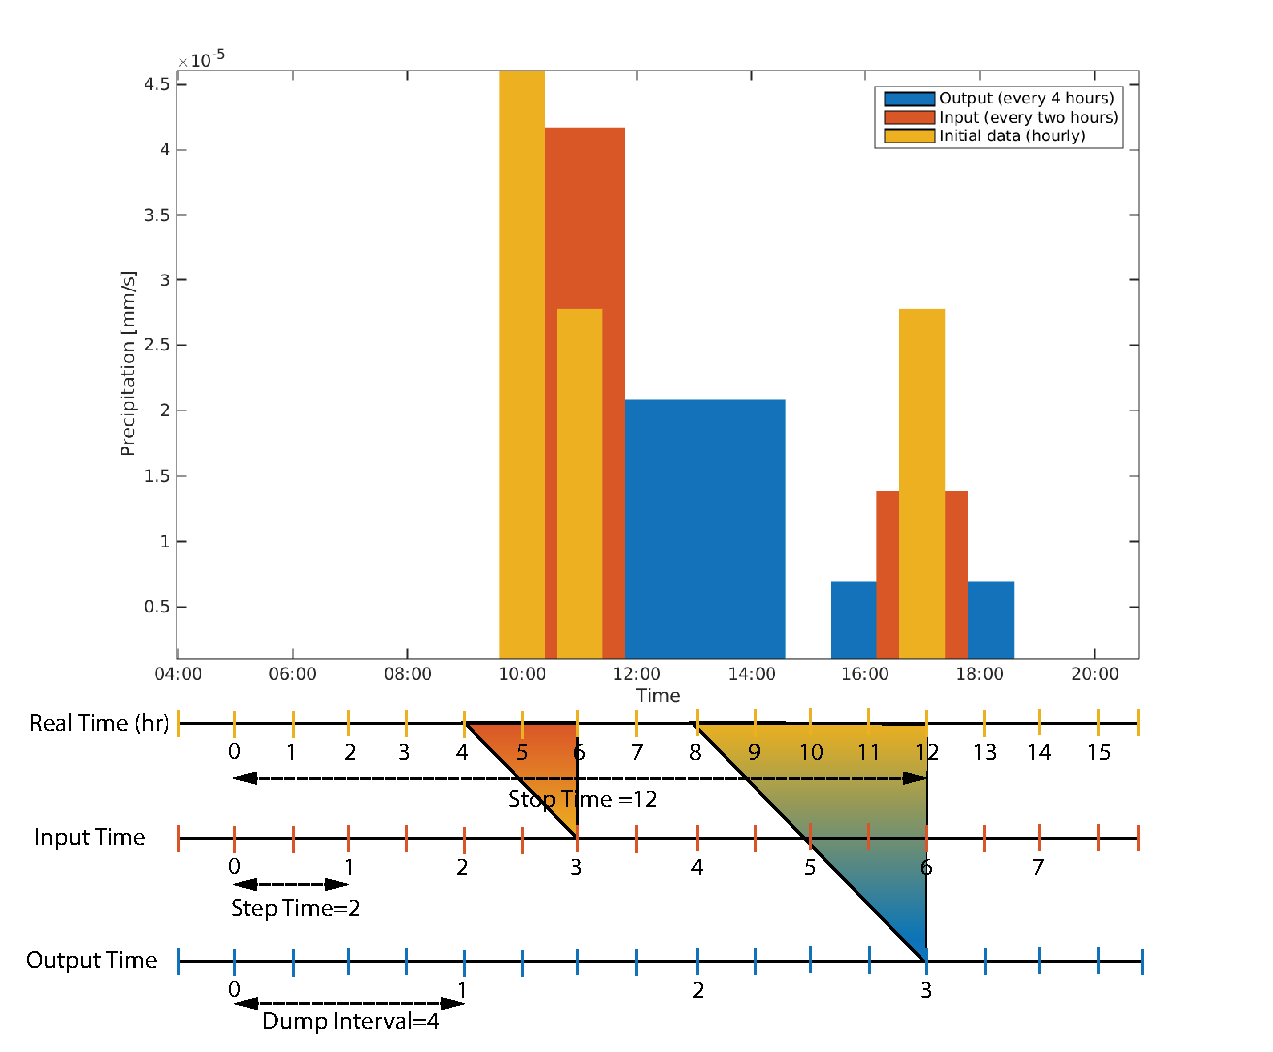
\includegraphics[width=\textwidth]{timeexplaination.eps}
\end{figure}


\section{Surface file}
Parflow needs 3 files related to the surface. You can fin python and fortran code helping you with that with \href{https://www.google.ca/url?sa=t&rct=j&q=&esrc=s&source=web&cd=1&ved=0CB4QFjAA&url=https%3A%2F%2Fusu.instructure.com%2Fcourses%2F127332%2Ffiles%2F27451190%2Fdownload%3Fwrap%3D1&ei=eTeqU-O2OMqj8QHO9IDYBw&usg=AFQjCNExTTlk9AMZ1GNuJWyUoWdywQuupQ&sig2=UsFhUrcWvzURS_92v-pACA&bvm=bv.69620078,d.b2U&cad=rja}{John Koudelka} or in an \href{http://igwmc.mines.edu/short-course/ParFlow/LW_example.pdf}{exemple of ParFlow}
\begin{itemize}
\item Slope X and Y.
	\begin{itemize}
	\item I think that I have understand that as the overlandflow is computed with the kinematic wave equation, flat zone or pit will arise in a large increase of water in this cell (peak). Parflow has a command to remove any flat ot local minima elevation. (see manual for more info). (be carfull, it needs to be a 4 cells not 8 cells as usual pit removal tools)
	\begin{lstlisting}[language=TCL]
set flatfill [pffillflats $dem]
set pitfill [pfpitfilldem $dem 0.01 50]
	\end{lstlisting}
	\end{itemize}
\item The solid file (.pfsol) is similar to a
Triangulated Irregular Network (TIN) but
includes subsurface layers beneath the dataset.
\end{itemize}


\end{document}
